\chapter{Image Based Profiling}

Modern fluorescence microscopy combined with high throughput biotechnology, automatically quantifying biological properties in images, is now widespread. They provide new insides into human cells and are powerful technologies for studying cell biology. 

More than  $10^{5}$ images can be produced per day. This makes automated image analysis mandatory for success. The aim of image-based profiling is to get as much data as possible from a biological sample and to encode it in a proper way. Image-based profiling experiments capture a wide range of data from a biological sample without prior knowledge of existence and use data mining and machine learning techniques in order to identify patterns.


\subsection{Drug Discovery}

One important application of image-based profiling is identifying biological machanism of actions (MOA). For example checking damage of DNA replication due to chemical perturbation. For developing new drugs and to make prediction about unknown chemical compounds it is important to know what chemical compounds cause which biological mechanism of action. Morphological profiles can predict these biological mechanisms of actions for chemical compounds.

\subsection{Typical Workflow}

There are two approaches in image-based phenotyping of perturbations. 
It should be considered that both fundamentally differ. The first approach includes phenotypic screening. Phenotypic screening focuses on pre-defined, specific phenotypes with the aim to identify drugs or drug targets that affect it.

The second way is profiling of perturbations. This approach profiles cells upon exposure to genetic, pathogenic or chemical perturbations.
Without further human intervention modern computer vision can extract features of cell morphology as cell size, shape, texture, intensity and many more.

\begin{figure}[H]
	\centering
	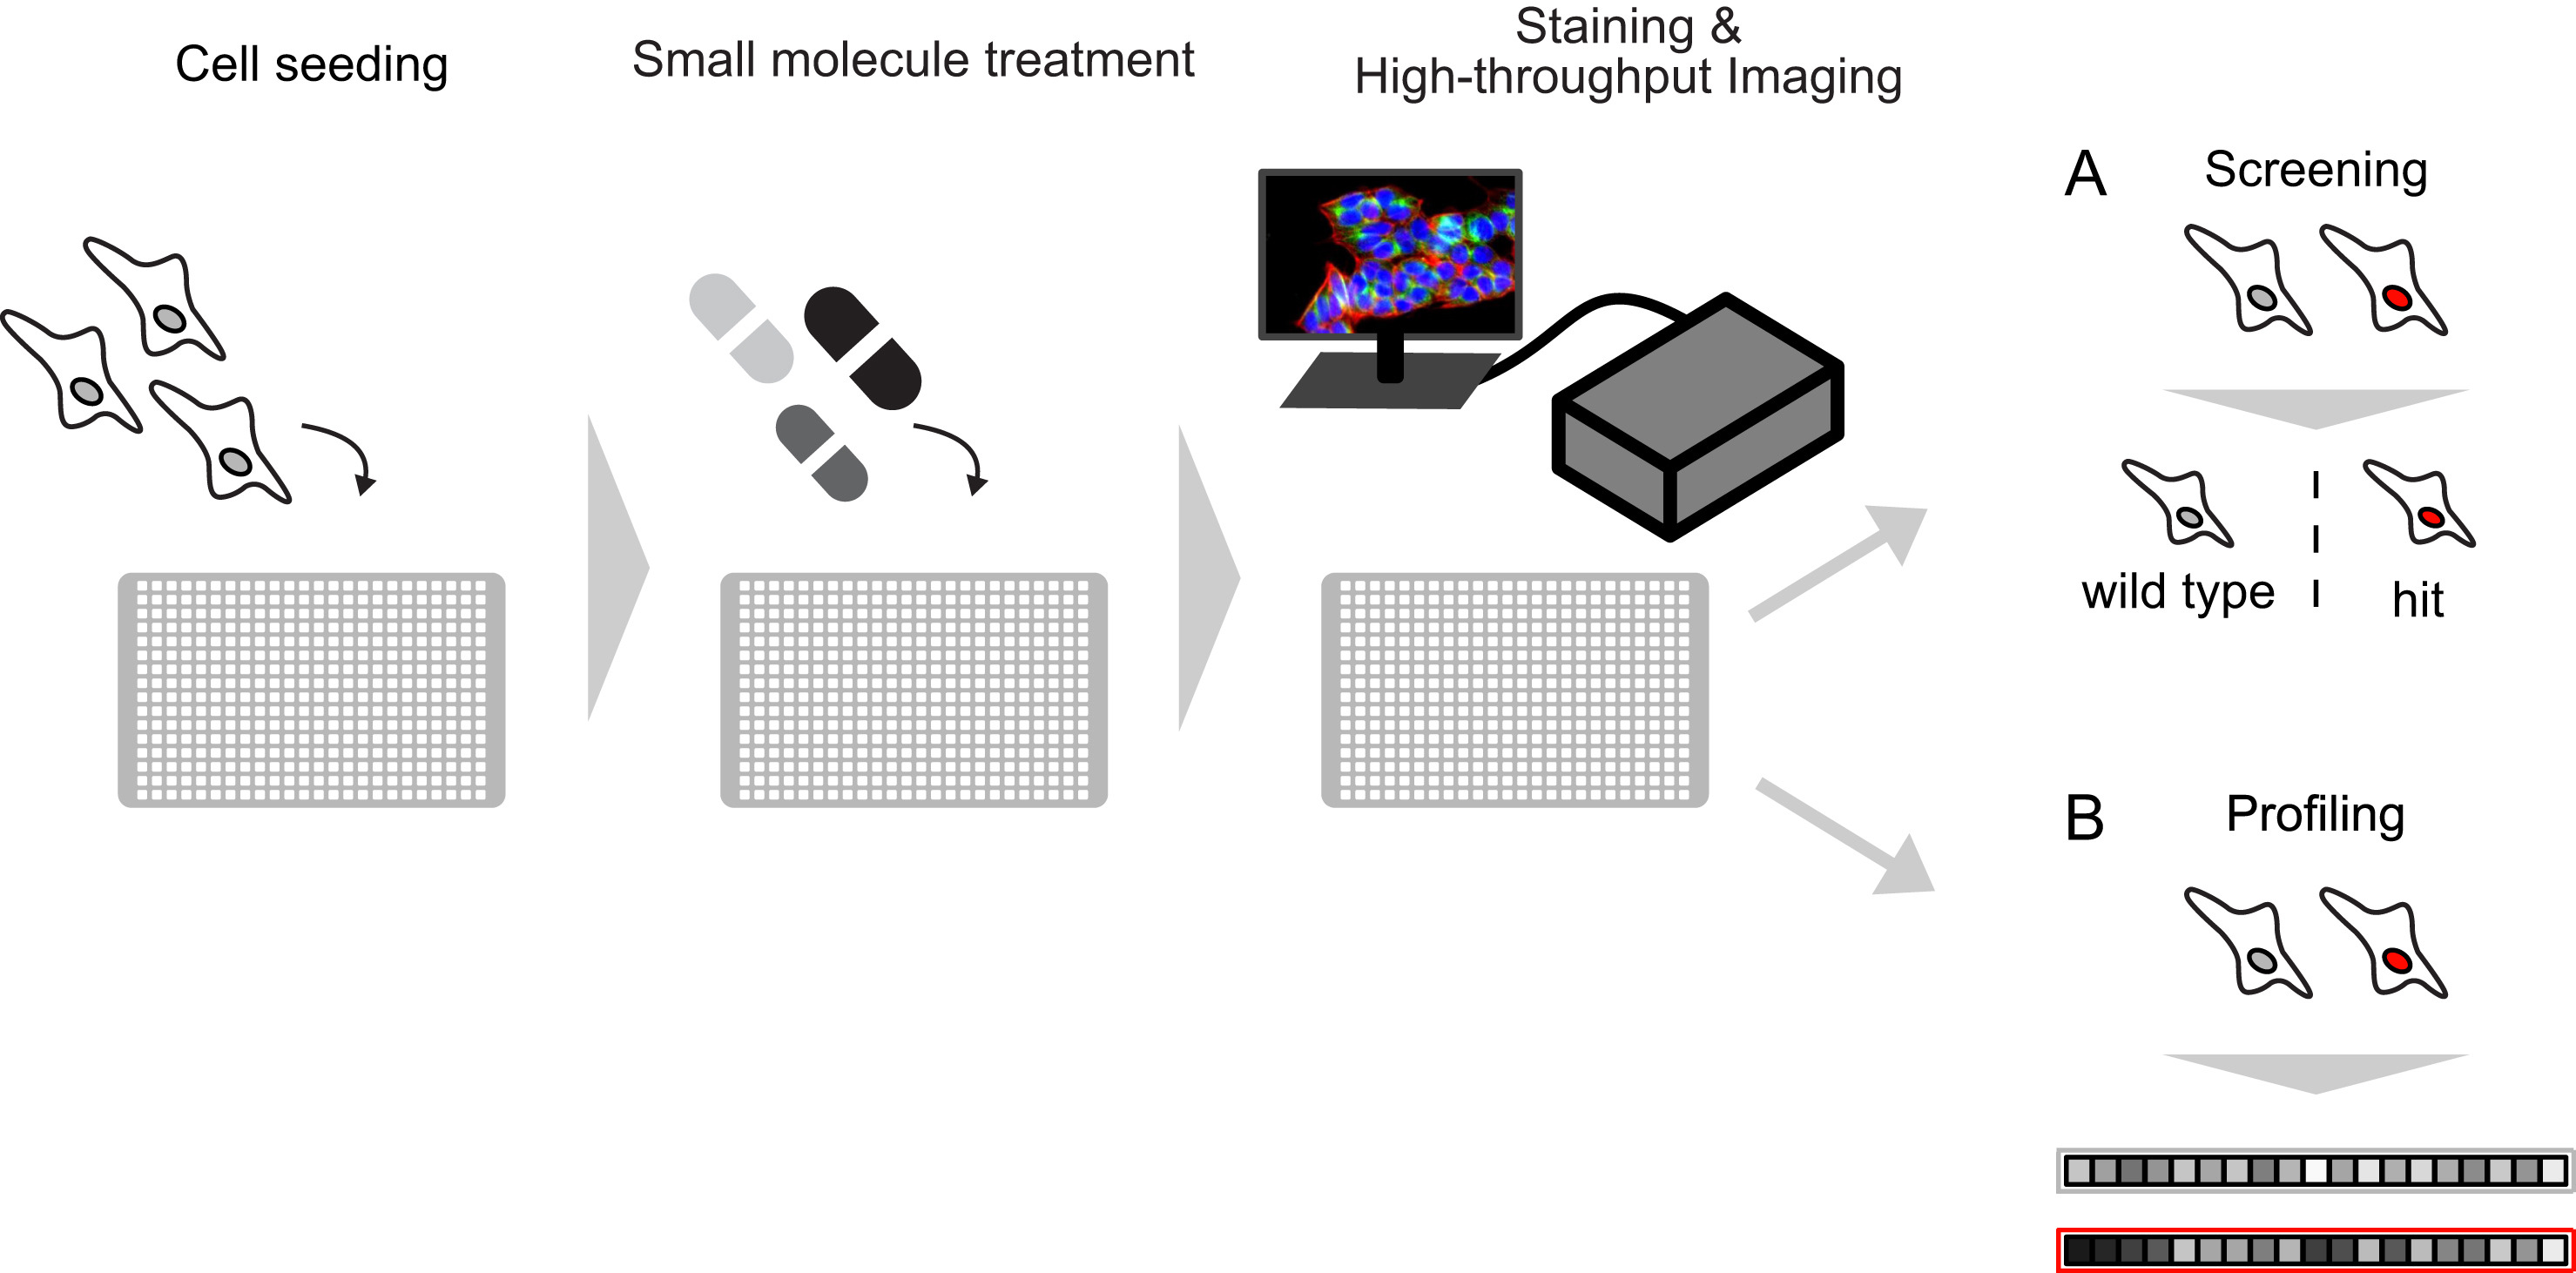
\includegraphics[width=0.8\linewidth]{bilder/cells/hcu.png}
	\caption{Typical workflow of image-based small molecule experiments. First cells need to be attached to plates. In a second step cells are perturbed. Then after staining the cells, images are taken using automated microscopes. At the end either screening approaches (A) or (B) profiling approaches can be used classify perturbed cells.}
	 source:\cite{Scheeder2018}
	\label{fig:Workflow}
\end{figure}

\subsubsection{Segmentation}

Small molecule profiling is based on staining subcellular structures.
An accurate segmentation of cells can be achieved by in intensity-based thresholding and other approaches. A number of computational applications for segmentation-free analysis in image-based profiling have been developed, the most famous one is Cell Profiler.


\begin{figure}[H]
	\centering
	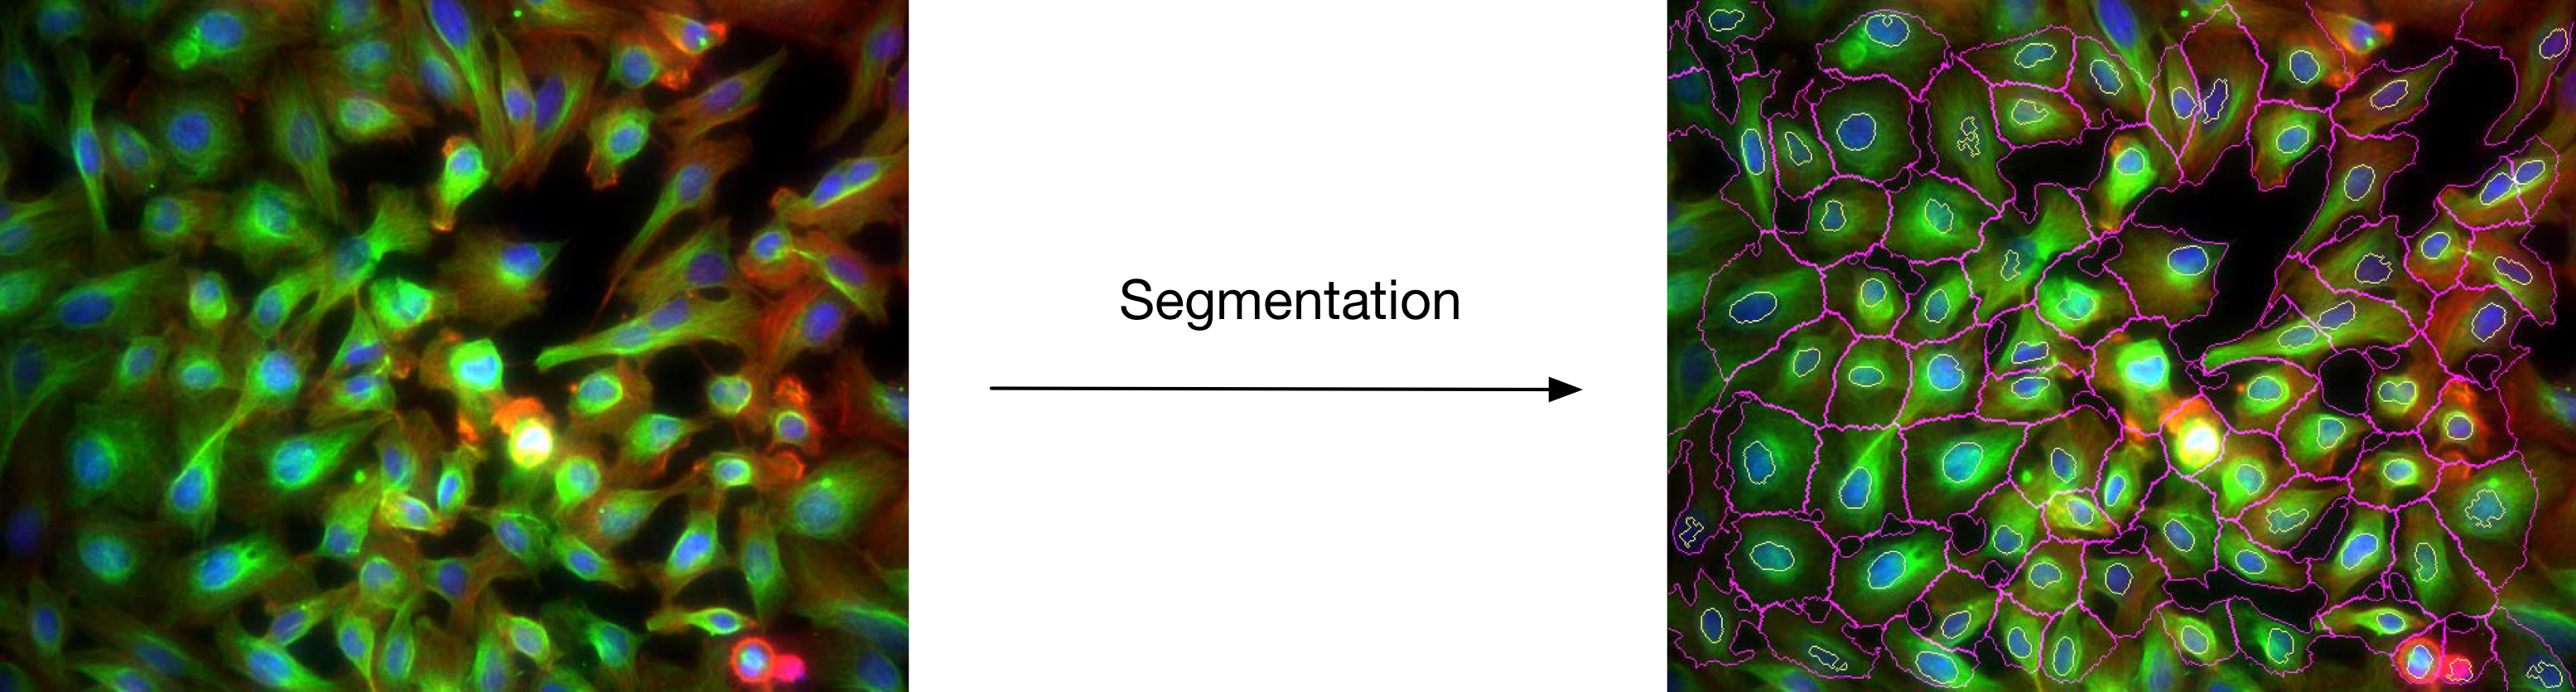
\includegraphics[width=0.8\linewidth]{bilder/cells/segmentation.png}
	\caption{Segmentation}
	source:\cite{Component}
	\label{fig:Segmentation}
\end{figure}


\subsubsection{Classification}


A typical aim for profiling experiments is the classification of compounds that cells have been perturbed with. Common classifiers are random forests or deep neural networks were employed in order to achieve higher accuracy in predicting biological machanism of actions.


\begin{figure}[H]
	\centering
	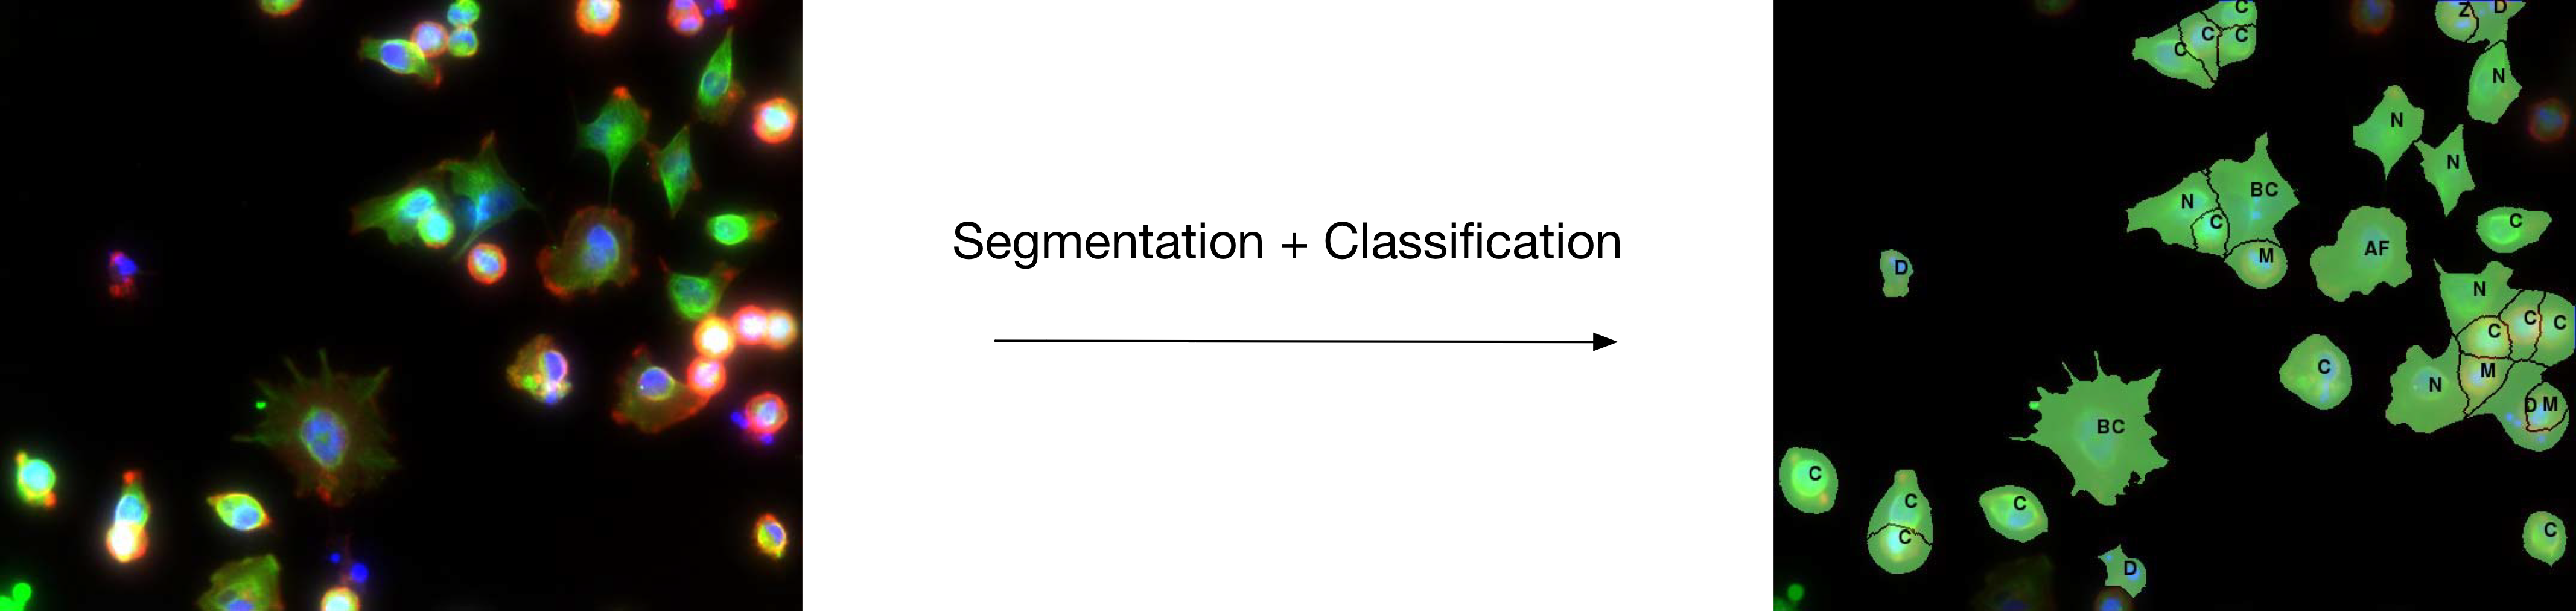
\includegraphics[width=0.8\linewidth]{bilder/cells/classification.png}
	\caption{Classification}
	source:\cite{Component}
	\label{fig:Classification}
\end{figure}




